\documentclass[Thesis.tex]{subfiles}
\begin{document}

\chapter{{\sc VaryLab} - Discrete surface optimization}
\label{chp:varylab}

\section{Introduction}

{\sc VaryLab} is a software developed at Berlin Institute of Technology by the author, Thilo R\"orig, and others. It is supported by DFG SFB/TRR 109 Discretization in Geometry and Dynamics. It is designed to be an extensible and modular tool for experiments with discrete surfaces in pure mathematics and applications in industrial geometry. {\sc VaryLab} is used to create the result in Chapters~\ref{chp:periodic_conformal_maps}, \ref{chp:quasiisothermic}, and \ref{chp:gridshells}.

In its core {\sc VaryLab} is a solver for non-linear optimization problems on the coordinates of a given 3D discrete surface. That means given a surface $S$ and functionals $f_1,\ldots,f_n:S\to\R$ we (try to) minimize the combined functional

\begin{eqnarray*}
	f(S) = \sum_{i=1}^n \lambda_i f_i(S)
\end{eqnarray*}
where $\lambda_1,\ldots,\lambda_n\in \R$ are user defined weights. 

{\sc VaryLab} uses the numerical library {\sc PETSc}/{\sc TAO} \cite{petsc-user-ref, petsc-web-page, tao-user-ref} and the corresponding {\sc Java} bindings \cite{jpetsctao-web-page} for computations. To run optimization methods we need at least an implementation of the functional's value. Other methods need gradient or Hessian of the functional. The most important methods are
 
\begin{tabular}{c | c | c}
	$S$ & $S$, $\nabla S$ & $S$, $\nabla S$, $\nabla\nabla S$\\ \hline
	{\tt NM} Nelder-Mead & {\tt LMVM} Limited-Memory, Variable-Metric & {\tt NLS} Newton Line-Search \\
	& {\tt CG} Conjugate Gradient & {\tt NTR} Newton Trust-Region.
\end{tabular}

In {\sc VaryLab} a functional can choose to implement just the value, see Section~\ref{sec:plugin-api}. Additionally it can implement the gradient and the Hessian of $S$. In principle all methods can be used with all functionals even if those do not implement all data needed for the algorithm. {\sc VaryLab} approximates the values of the gradient or the Hessian if they are missing. 

Derivatives and numerical substitutes, 
Boundary Conditions
Numerics
Build-In Functionals
Plug-in facility and extensibility, 
Data Visualization (scalar, vector)
Remeshing

\begin{figure}
\begin{center}
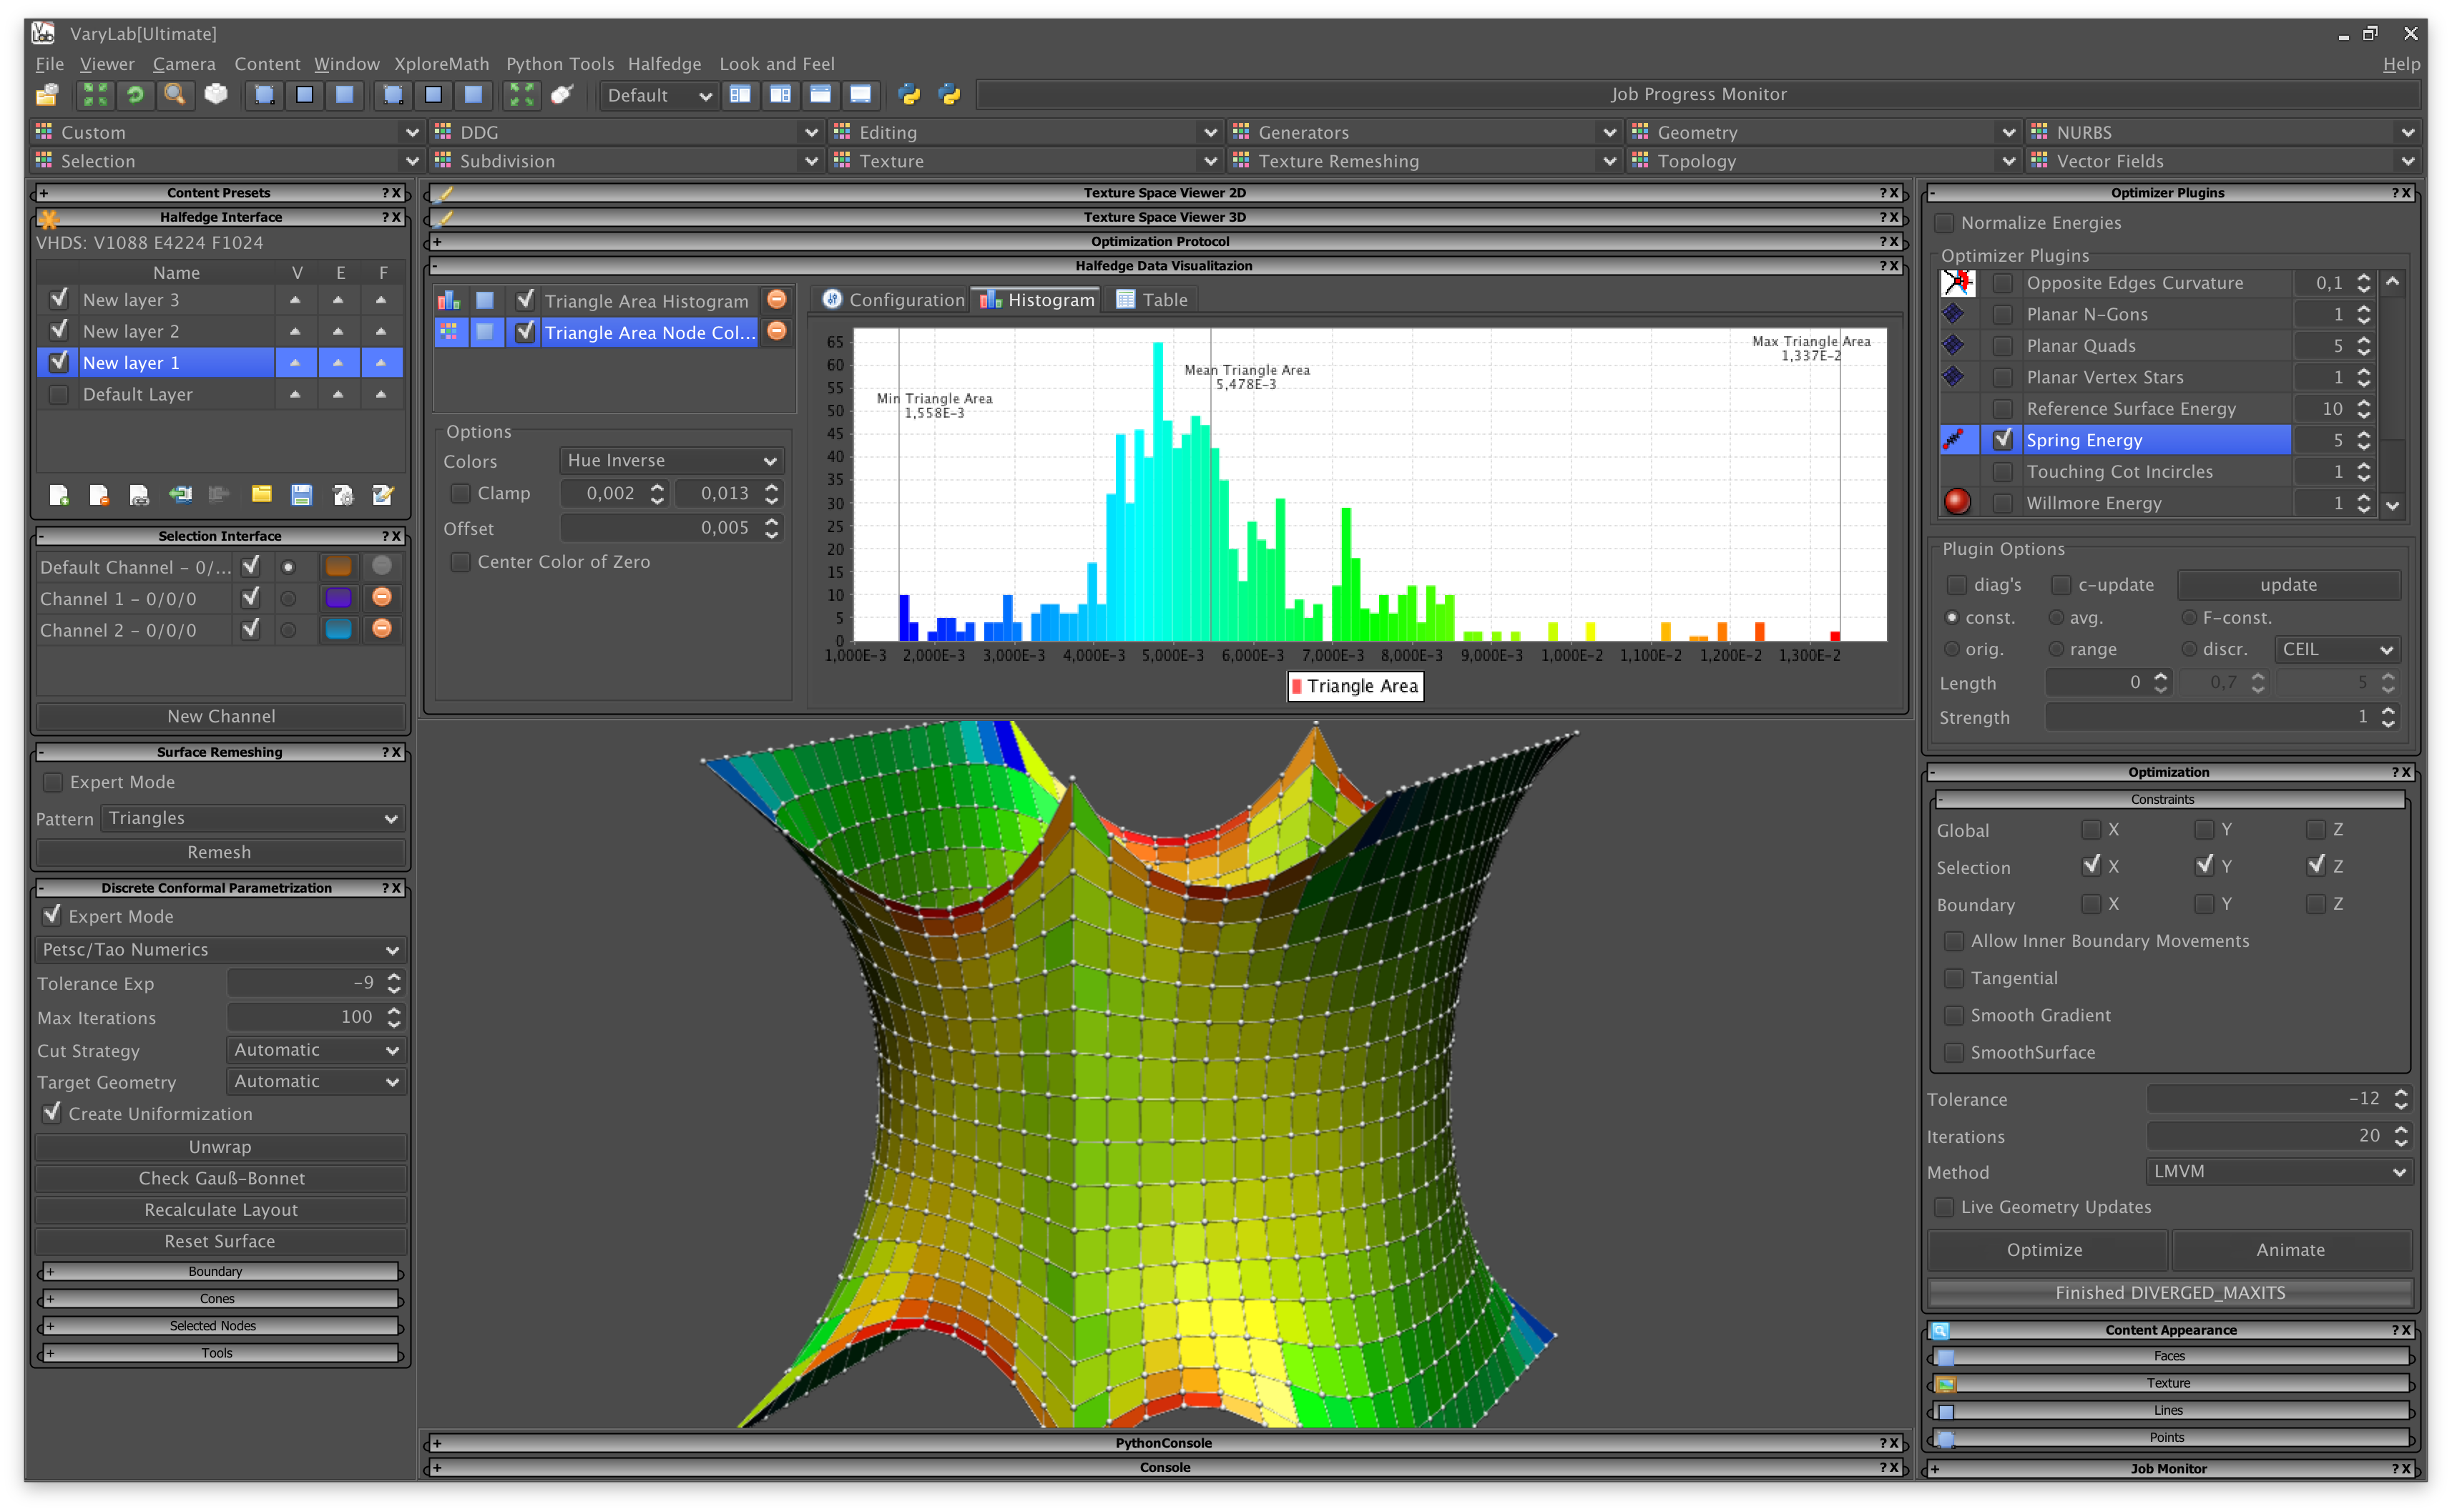
\includegraphics[width=\textwidth]{varylab/varylab_main.png}
\caption{{\sc VaryLab} user interface.}
\label{fig:varylab_main_ui}
\end{center}
\end{figure}

\section{Plug-in API}
\label{sec:plugin-api}

\section{User interface}



\begin{figure}
\begin{center}
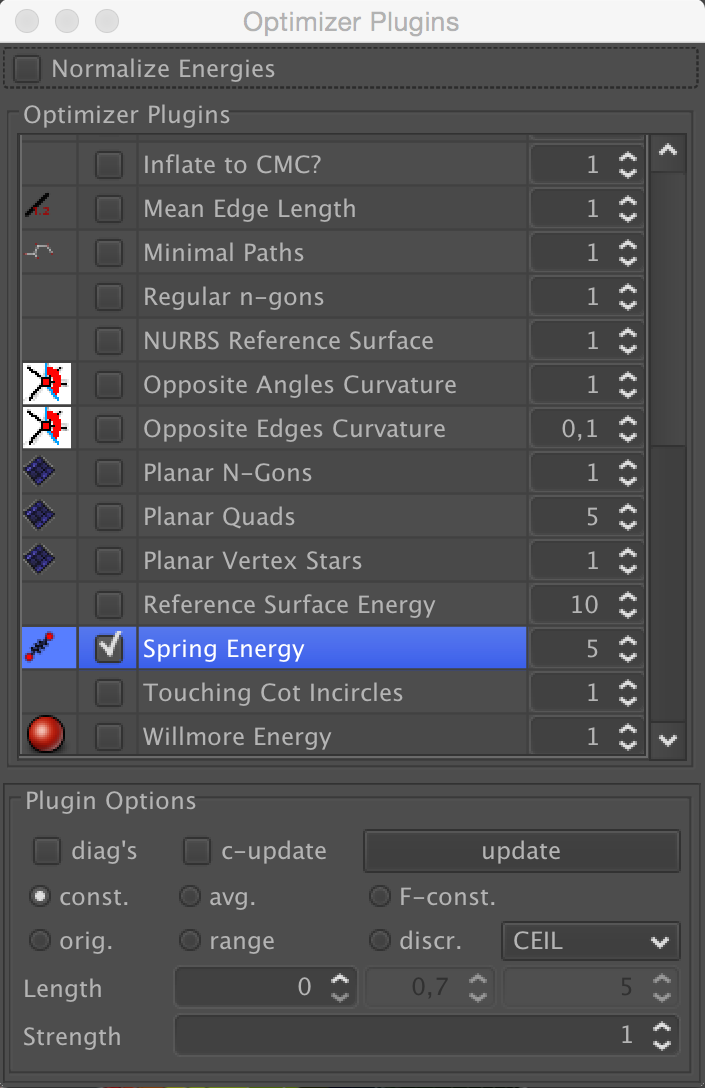
\includegraphics[width=0.5\textwidth]{varylab/optimization_plugins.png}\hfill
\begin{minipage}[b]{0.47\linewidth}
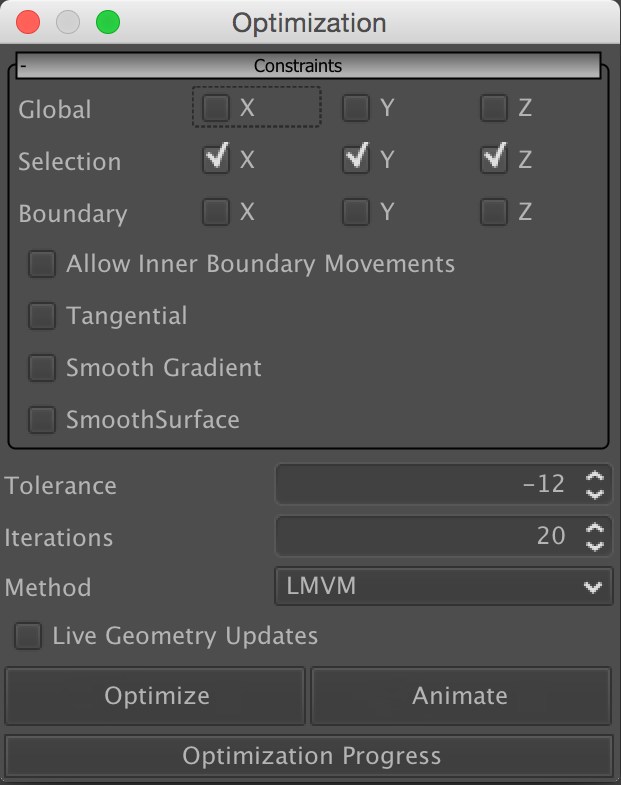
\includegraphics[width=\linewidth]{varylab/optimization.png}\\
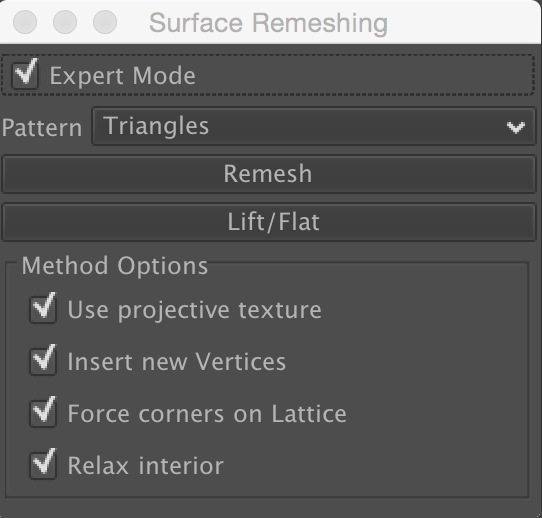
\includegraphics[width=\linewidth]{varylab/remeshing.png}
\end{minipage}\\
\vskip 0.05cm
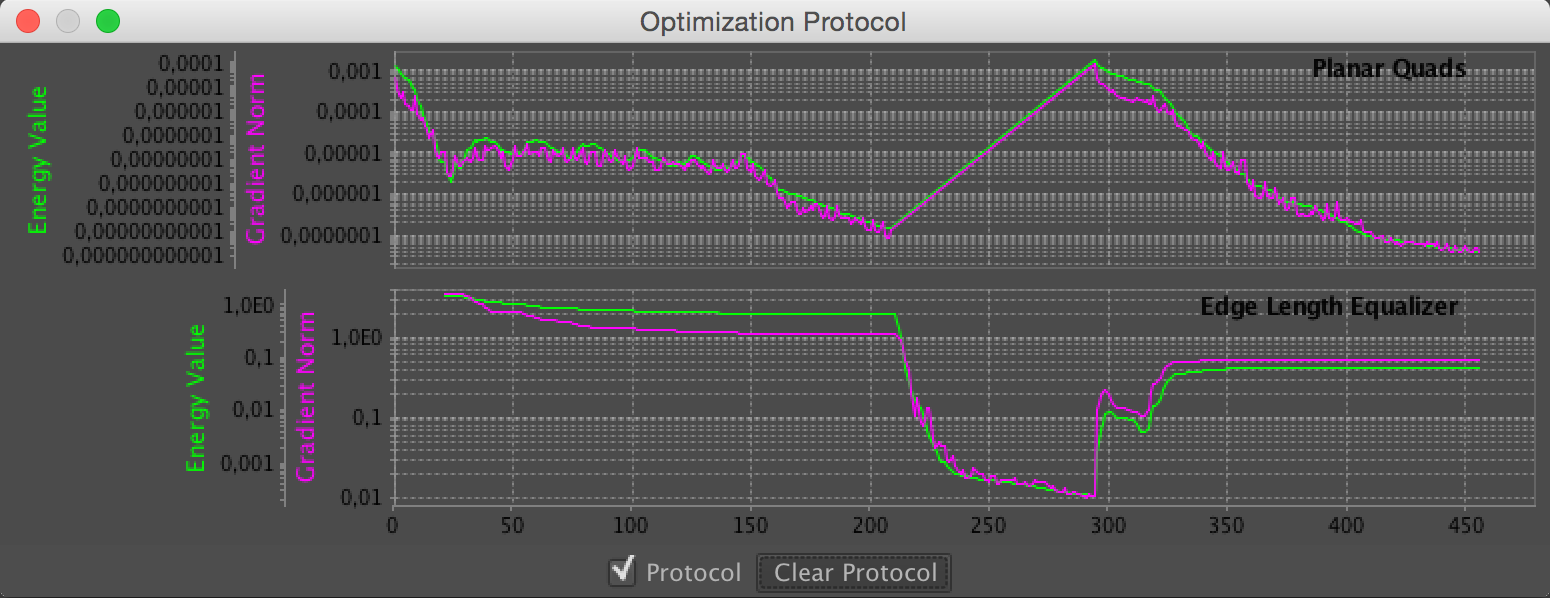
\includegraphics[width=\textwidth]{varylab/protocol.png}
\caption{The main user interface panels of {\sc VaryLab}. List of optimization functional plug-ins and their options (left). Main optimization controls with global constraints and minimizer settings (top right). Remeshing ui for different patterns (right middle). Optimization protocol panel (bottom) shows the progress of the optimization for each activated energy.}
\label{default}
\end{center}
\end{figure}



\section{{\sc VaryLab[Service]}}


\section{Periodic conformal maps with {\sc VaryLab}}
In this section we describe how the methods described in Chapter~\ref{chp:periodic_conformal_maps} are implemented in {\sc VaryLab} and {\sc ConformalLab}. 

The parameterization part of the work is carried out via the {\sc ConformalLab} main user interface. 

Load a model with two boundary components. 

\section{{\sc U3D} - 3D content in presentations and online publications}
\label{sec:u3d}

\subfilebibliography
\end{document}

%%% Local Variables:
%%% TeX-master: "Thesis.tex"
%%% End: